
Uma série estatística consiste em um conjunto de dados organizado com base em uma característica comum, ou seja, uma mesma variável. Normalmente, uma série estatística é representada por meio de uma tabela ou de um gráfico, conforme ficar melhor representado, a fim de sintetizar os dados estatísticos observados e torná-los mais compreensivos.

\begin{enumerate}[label=\alph*.]
    \item Corpo — conjunto de linhas e colunas com as informações sobre a variável em estudo;
    \item cabeçalho — parte superior que especifica o conteúdo das colunas;
    \item coluna indicadora — parte que indica o conteúdo das linhas;
    \item linhas — traços que facilitam a leitura dos dados;
    \item célula — espaço onde os dados são armazenados;
    \item título — identificação da tabela, contendo as informações sobre seu conteúdo;
    \item fonte — referência de onde os dados foram obtidos, localizada no rodapé.
\end{enumerate}
\begin{figure}[H]
    \begin{center}
        \includegraphics[width=.8\linewidth]{Estat_01.png}

    \end{center}
    \caption{Série estatística}
\end{figure}

Um gráfico é uma forma clara e objetiva de apresentar uma série estatística. O objetivo é proporcionar uma compreensão mais rápida do fenômeno em estudo. Para isso, o gráfico deve ser destituído de detalhes sem importância (ser simples); permitir a correta intepretação dos valores representativos do fenômeno (ser
claro); e transmitir a verdade sobre o fenômeno (ser verossímil). A série estatística apresentada na tabela anterior pode ser representada graficamente da seguinte forma:
\begin{figure}[hbt]
  \centering
  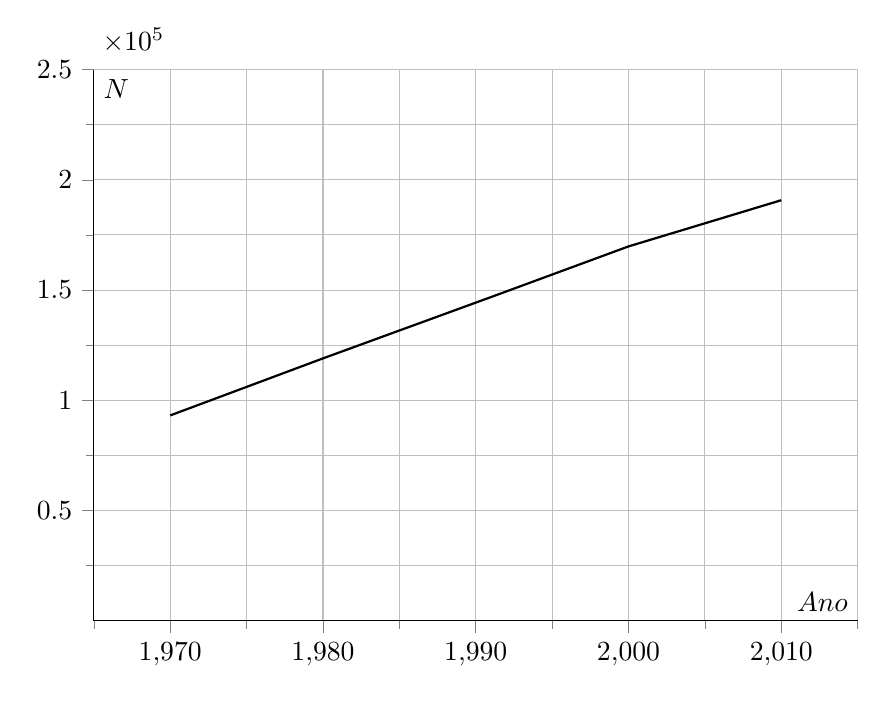
\begin{tikzpicture}
    \begin{axis}[
    xmin=1965, xmax=2015,
    ymin=0, ymax=250000,
    axis x line=middle,
    axis y line=middle,
    width=0.8 \textwidth,
    height=7cm,
    scale only axis,
    scaled y ticks=true,
    ytick scale label code/.code={$\times 10^{#1}$},
    xtick distance=10, % ajuste: 5, 10, 20...
      axis line style={-},
      tick align=outside,
      grid=both,
      minor tick num=1,
      xlabel={$Ano$},
      ylabel={$N$},
    ]
           \addplot[
        thick
      ] coordinates {
        (1970,93143)
        (1980,119011)
        (1991,146825)
        (2000,169799)
        (2010,190755)
      };
    \end{axis}
  \end{tikzpicture}
  \caption{Variação da População.}
\end{figure}

  Tabela.
  \begin{itemize}
    \item Quadro que resume um conjunto de observações.
    \item Composta de cabeçalho, corpo, coluna indicadora, linhas, células, título e fonte.
  \end{itemize}
  Gráfico.
  \begin{itemize}
    \item Forma simples e clara de apresentar uma série estatística.
    \item Proporcionar uma compreensão mais rápida do fenômeno em estudo.
    \item Deve ser simples, claro e verossímil.
  \end{itemize}
Finalmente, podemos verificar a presença de três elementos nas séries estatísticas: o tempo, o espaço e a espécie. Conforme os elementos variem, a série pode ser classificada em temporal (ou cronológica), geográfica (ou territorial) e específica.

\subsection{Séries Temporais (cronológicas)}

É a série cujos dados são dispostos segundo a época de ocorrência. Isto é, enquanto o tempo varia, o fato e o local permanecem constantes. Também são chamadas de séries históricas ou evolutivas. A principal característica é o fator cronológico variável.

A seguir temos a série histórica da população residente no Brasil no período de 1970 a 2010, com frequência decenal. Percebam que o tempo varia; contudo, o fato que está sendo analisado (quantidade populacional) e o local alvo da pesquisa (Brasil), continuam iguais.

\begin{table}[H]
    \centering
    \begin{tabular}{ll}
        \toprule
      Anos  &   População\\
      1970  &   93143\\
      1980  &   119011\\
      1991  &   146825\\
      2000  &   169799\\
      2010  &   190755\\
        \midrule
        \bottomrule
          \end{tabular}
    \caption{Censo 2010}
\end{table}

\subsection{Séries Geográficas (ou Territoriais)}
É a série cujos dados são dispostos segundo a localidade de ocorrência. Isto é, enquanto o local varia, o fato e o tempo permanecem constantes. Também são chamadas de séries espaciais ou de localização. A principal característica é o fator geográfico variável.

A seguir temos a série geográfica da população urbana residente em cada uma das regiões brasileiras no ano de 2010. Percebam que o local (região) varia; contudo, o fato que está sendo analisado (quantidade populacional) e o tempo (ano de 2010) permanecem constantes.


\begin{table}[H]
    \centering
    \begin{tabular}{ll}
        \toprule
      Região    &       População\\
      norte         &   11664\\
      nordeste      &   32821\\
      sudeste       &   74696\\
      sul           &   23260\\
      centro-oeste  &   12482\\
        \midrule
        \bottomrule
          \end{tabular}
    \caption{Censo 2010}
\end{table}

\subsection{Séries Específicas}

É a série cujos dados são dispostos segundo a modalidade de ocorrência. Isto é, enquanto o fato varia, a época e o local permanecem constantes. Também são chamadas de séries categóricas. A principal característica é o fator especificativo variável.

A seguir temos uma série específica das populações urbana e rural residentes no Brasil no ano de 2010. Percebam que os fatos analisados variam (população urbana x população rural); contudo, o tempo (2010) e o local de análise (Brasil) são onstantes.

\begin{table}[H]
    \centering
    \begin{tabular}{ll}
        \toprule
      Zona    &   População\\
      Urbano  &   93134\\
      Rural   &   119011\\
         \midrule
        \bottomrule
          \end{tabular}
    \caption{Censo 2010}
\end{table}

\subsection{Séries Mistas (ou Compostas)}

Muitas vezes, podemos ter a necessidade de apresentar, em uma única tabela, a variação de valores de mais de uma variável, isto é, combinar duas ou mais séries. As séries resultantes desse processo de combinação são chamadas de séries mistas (ou compostas) e apresentadas por meio de tabelas de dupla entrada.

O nome da nova série deve considerar pelo menos dois elementos. Assim, se for uma série mista de fato e tempo, denominaremos de série específico-temporal. A seguir temos uma série específicotemporal representando as populações de homens e mulheres residentes no Brasil, no período de 1970 a 2010, com variação decenal.

\begin{table}[H]
  \centering
  \caption{População residente no Brasil por sexo (1970--2010).}
  \label{tab:censo_sexo_1970_2010}
  \begin{tabular}{lrr}
    \toprule
      \multicolumn{1}{c}{} & \multicolumn{2}{c}{Sexo} \\
      \cmidrule(lr){2-3}
      \multicolumn{1}{c}{Ano} & \multicolumn{1}{c}{Homens} & \multicolumn{1}{c}{Mulheres} \\
    \midrule
    1970 & 46327 & 46807 \\
    1980 & 59142 & 59868 \\
    1991 & 72485 & 74340 \\
    2000 & 83602 & 86270 \\
    2010 & 93406 & 97348 \\
    \bottomrule
  \end{tabular}
\end{table}

Por sua vez, se tivermos uma série mista de local e tempo, denominaremos de série geográfica-temporal.
A seguir temos uma série geográfico-temporal representando as populações residentes em cada região brasileira, no período de 1970 a 2010, com variação decenal.

\begin{table}[H]
  \centering
  \begin{tabular}{lrrrrr}
    \toprule
      & \multicolumn{5}{c}{Regiões} \\
      \cmidrule(lr){2-6}
    Anos & N & NE & SE & S & CO \\
    \midrule
    1970 & 3105  & 28111 & 3980  & 16496 & 5072 \\
    1980 & 5880  & 34815 & 51737 & 19031 & 7545 \\
    1991 & 10030 & 42497 & 62470 & 22129 & 9427 \\
    2000 & 12900 & 47741 & 72412 & 25107 & 11636 \\
    2010 & 15864 & 53081 & 80364 & 27386 & 14058 \\
    \bottomrule
  \end{tabular}
  \caption{Censo 2010}
\end{table}

Por fim, devemos notar que podem existir séries compostas de três ou mais entradas, embora isso raramente aconteça, por conta da dificuldade de representação.